% Q06 -- System timing: two-phase NON-OVERLAPPING clock (phi1 leads phi2, never both high).
% From the notes: phi1 and phi2 are the system clocks; writes Anded with phi1, refresh on phi2.
\documentclass[border=10pt]{standalone}
\usepackage{tikz}
\usetikzlibrary{arrows.meta}
\begin{document}
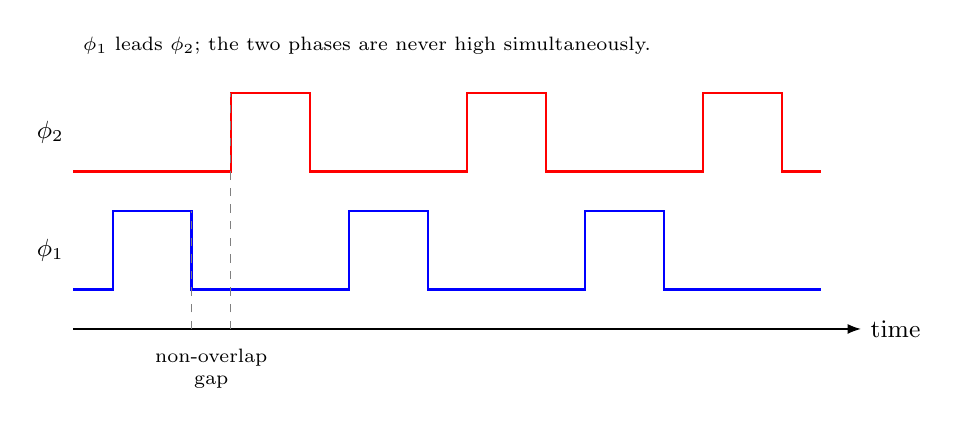
\begin{tikzpicture}[>=Latex, font=\small, x=0.5cm, y=0.5cm]
% time axis
\draw[->] (0,-1) -- (20,-1) node[right]{time};
% phi1 : high during [1,3], [7,9], [13,15]
\node[left] at (0,1) {$\phi_1$};
\draw[thick, blue]
  (0,0) -- (1,0) -- (1,2) -- (3,2) -- (3,0) --
  (7,0) -- (7,2) -- (9,2) -- (9,0) --
  (13,0) -- (13,2) -- (15,2) -- (15,0) -- (19,0);
% phi2 : high during [4,6], [10,12], [16,18]  (never overlaps phi1, lags phi1)
\node[left] at (0,4) {$\phi_2$};
\draw[thick, red]
  (0,3) -- (4,3) -- (4,5) -- (6,5) -- (6,3) --
  (10,3) -- (10,5) -- (12,5) -- (12,3) --
  (16,3) -- (16,5) -- (18,5) -- (18,3) -- (19,3);
% guard-band markers showing non-overlap between phi1 fall and phi2 rise
\draw[dashed, gray] (3,-1) -- (3,2);
\draw[dashed, gray] (4,-1) -- (4,5);
\node[font=\scriptsize, align=center] at (3.5,-2.0) {non-overlap\\ gap};
\node[font=\scriptsize, anchor=west] at (0,6.2)
  {$\phi_1$ leads $\phi_2$; the two phases are never high simultaneously.};
\end{tikzpicture}
\end{document}
